\documentclass[preprint,12pt]{elsarticle}

\usepackage[T1]{fontenc}
\usepackage[utf8]{inputenc}
\usepackage{graphicx}
\usepackage{amsmath,amssymb}
\usepackage{booktabs}
\usepackage{multirow}
\usepackage{tabularx}
\usepackage{array}
\usepackage{algorithm}
\usepackage{algpseudocode}
\usepackage{siunitx}
\usepackage{xcolor}
\usepackage{tikz}
\usetikzlibrary{positioning,arrows.meta}
\usepackage{hyperref}
\hypersetup{hidelinks}
\usepackage{url}

\graphicspath{{./Figures/}{Figures/}{../Figures/}{../../Figures/}{../../../Figures/}}
\sisetup{round-mode=places,round-precision=3}
\setlength{\textfloatsep}{5pt plus 1pt minus 1pt}
\setlength{\floatsep}{5pt plus 1pt minus 1pt}
\setlength{\intextsep}{5pt plus 1pt minus 1pt}
\setlength{\abovecaptionskip}{4pt}
\setlength{\belowcaptionskip}{0pt}
\setlength{\abovedisplayskip}{6pt plus 1pt minus 1pt}
\setlength{\belowdisplayskip}{6pt plus 1pt minus 1pt}
\setlength{\abovedisplayshortskip}{4pt plus 1pt minus 1pt}
\setlength{\belowdisplayshortskip}{4pt plus 1pt minus 1pt}
\setlength{\emergencystretch}{3em}
\setcounter{topnumber}{3}
\setcounter{totalnumber}{5}
\renewcommand{\topfraction}{0.95}
\renewcommand{\textfraction}{0.05}
\renewcommand{\floatpagefraction}{0.85}
\raggedbottom

\begin{document}

\begin{frontmatter}

\title{ADARE: Pareto-Contextual Adaptive Control for Many-Objective Workflow Scheduling in Heterogeneous Edge/Fog/Cloud Systems}

\author[cyu]{Roland Cedric Tayo\corref{cor1}}
\ead{rolandcedric.tayo@yahoo.fr}
\author[cyu]{Sonia Yassa}
\ead{sonia.yassa@cyu.fr}
\cortext[cor1]{Corresponding author.}
\address[cyu]{CY Cergy Paris University, France}

\begin{abstract}
ADARE (Adaptive Data-driven Algorithm for Resource Evolution) is an adaptive extension of NSGA-III for four-objective Edge/Fog/Cloud workflow scheduling. It retains NSGA-III reference-vector environmental survival and adds a contextual controller over four crossover operators, density-aware mutation, bounded archive injection, and auditable decision traces. The controller state combines search phase, population diversity, and stagnation; its bounded reward combines Pareto dominance, range-normalized improvement, balanced objective progress, and genotype novelty. We evaluate the extension under matched seeds, initial populations, evaluators, and generation/population budgets. Across the small-workflow comparison, ADARE has favorable paired effects in 81 of 90 algorithm--benchmark--indicator comparisons. At 1000 tasks it is favorable in 78/80 comparisons at 50 generations and 69/80 at 100 generations; 56 and 55, respectively, remain significant after Holm correction. At the 3000-task class it is favorable in 88/100 comparisons, with 33 Holm-significant. QL-NSGA-III remains competitive under longer budgets, so these results do not establish universal superiority. Across 20 independent runs, immediate reward correlates positively with offspring survival (mean Spearman $\rho=0.32$ on CyberShake and $0.27$ on Montage). Controller selection uses about 0.27\% of runtime and reward/update operations about 4.8\%. Evaluation/time trajectories, sampled process-tree memory, and three resource configurations further delimit the empirical scope. The evidence supports ADARE as a transparent, workflow-tailored adaptive-control layer for NSGA-III rather than a new environmental-selection algorithm.
\end{abstract}

\begin{keyword}
Online learning \sep Many-objective optimization \sep Adaptive operator selection \sep Multi-armed bandits \sep Edge/Fog/Cloud \sep Workflow scheduling
\end{keyword}

\end{frontmatter}

\section{Introduction}
\begin{sloppypar}
Modern distributed applications execute over heterogeneous edge, fog, and cloud resources with different compute rates, bandwidths, prices, and power levels. Mapping a precedence-constrained workflow onto these resources creates conflicting makespan, latency, cost, and energy objectives. The execution model studied here is deterministic: resource attributes and task sizes are fixed within a run. Randomness enters through the evolutionary search, not through node failures or time-varying systems behavior.
\end{sloppypar}

NSGA-III reference-vector survival provides a strong and interpretable many-objective backbone \cite{deb2014nsga3}, but its standard variation schedule is static. A crossover useful during early exploration need not remain useful after diversity contracts or progress stalls. ADARE addresses this narrower question: can search-state feedback adapt variation around an otherwise unchanged NSGA-III survival mechanism? We therefore position ADARE explicitly as \emph{NSGA-III with workflow-tailored adaptive operator control}, not as an unrelated environmental-selection method.

\paragraph{Motivation and methodological gap.}
Adaptive operator selection, parameter control, and UCB are established ideas \cite{auer2002ucb,dacosta2008aos,fialho2010aos,karafotias2015parameter}; their mere combination is not our novelty claim. The unresolved design problem is operational: which inexpensive state and reward signals can be computed for every mating event in a four-objective DAG scheduler, remain invariant to objective units, and be audited against downstream survival? ADARE specializes the state to phase/diversity/stagnation regimes and the reward to Pareto-normalized parent--offspring evidence. Density-aware assignment mutation and bounded archive injection provide workflow-specific recovery mechanisms around that controller.

\paragraph{Contributions.}
The contributions are:
\begin{enumerate}
    \item an operational 12-context controller with four precisely specified crossover actions and a bounded, range-normalized Pareto reward;
    \item workflow-tailored density-aware assignment mutation, local repair, and bounded archive injection around unchanged NSGA-III survival;
    \item controlled controller/reward ablations, reward--survival validation, and complete paired inference with one-sided Wilcoxon tests, Holm correction, paired rank-biserial effects, and bootstrap confidence intervals;
    \item repeated small, 1000-task, and 3000-task experiments, including a 100-generation pressure test and convergence against objective evaluations and wall-clock time; and
    \item explicit runtime, process-tree memory, and resource-configuration sensitivity analyses that bound rather than overstate scalability and generalizability.
\end{enumerate}

% Author reasoning clarification
The remainder of this paper is structured as follows: Section 2 reviews related work, Section 3 presents the problem modeling, Section 4 describes the proposed approach, and Section 5 details the experimental protocol and experimental results. Section 6 discusses the findings and their limitations, and Section 7 concludes the paper and outlines future research directions.

\section{Related Work}
\subsection{Heterogeneous workflow scheduling}
Workflow scheduling maps a DAG onto heterogeneous resources while respecting precedence, serialization, and communication delays. HEFT remains a relevant low-cost makespan heuristic \cite{topcuoglu2002heft}, but a single priority list does not directly represent four-way latency, cost, energy, and completion-time trade-offs. Public Pegasus and WfCommons workflows support reproducible evaluation across application structures and scales \cite{pegasus,coleman2021wfcommons}.

\subsection{Many-objective survival and adaptive variation}
NSGA-II, NSGA-III, and MOEA/D represent dominance-, reference-vector-, and decomposition-based search, respectively \cite{deb2002nsga2,deb2014nsga3,zhang2007moead}. ADARE inherits NSGA-III environmental survival; its comparison with static NSGA-III therefore measures the surrounding adaptive-control layer while holding survival fixed. Bandit-based adaptive operator selection predates this work \cite{dacosta2008aos,fialho2010aos}, and recent surveys describe a broad range of reinforcement-learning-assisted evolutionary mechanisms \cite{song2024survey}.

OVEA uses Q-learning for crossover choice with reference-vector selection \cite{jiao2023ovea}; MRL-MOEA uses multiple search states to select operators \cite{wang2025mrlmoea}; and QMOEA/D-AWA adapts decomposition neighborhoods for low-carbon flexible job-shop scheduling \cite{wang2026qmoeadawa}. DRLMMEA targets multimodal multi-objective optimization with deep-RL-guided operator selection \cite{cui2026drlmmea}. These methods motivate stronger adaptive baselines but solve different encodings and, in several cases, different problem classes. Our OVEA-style and QMOEA/D-AWA-style implementations are therefore declared workflow adaptations, not verified reproductions of the published algorithms; we do not claim to outperform the original families. Exact public-artifact transfer and a multiobjective HEFT family remain external-validity work.

\subsection{Positioned contribution}
The methodological contribution is the jointly operationalized state/reward/mutation design around NSGA-III for a deterministic heterogeneous DAG evaluator. Phase, diversity, and stagnation provide 12 auditable contexts; reward is computed from unit-normalized Pareto evidence; and every controller action can be linked to offspring survival. Controlled ablations test whether that controller adds evidence beyond static or global selection under identical mutation/archive settings. Detailed baseline adaptations and parameter settings are moved to the experimental protocol rather than repeated here.

\section{Problem Modeling}
\subsection{System Model}
We consider a workflow represented as a directed acyclic graph (DAG) $G=(V,E)$, where each task $v_i \in V$ carries a computational load and a data transfer footprint, and each directed edge encodes a precedence relation with communication dependency. The execution platform is a heterogeneous resource set $R$ spanning edge, fog, and cloud nodes, each characterized by processing rate, communication bandwidth, monetary processing cost, and power usage.

A candidate schedule is encoded as a task-to-node assignment vector
\begin{equation}
x=(x_1,\ldots,x_{|V|}), \qquad x_i \in \{0,1,\ldots,|R|-1\}.
\end{equation}
Given a topological order of the DAG, the evaluator simulates task start and finish times under node availability and inter-node transfer delays.

\begin{figure}[t]
\centering
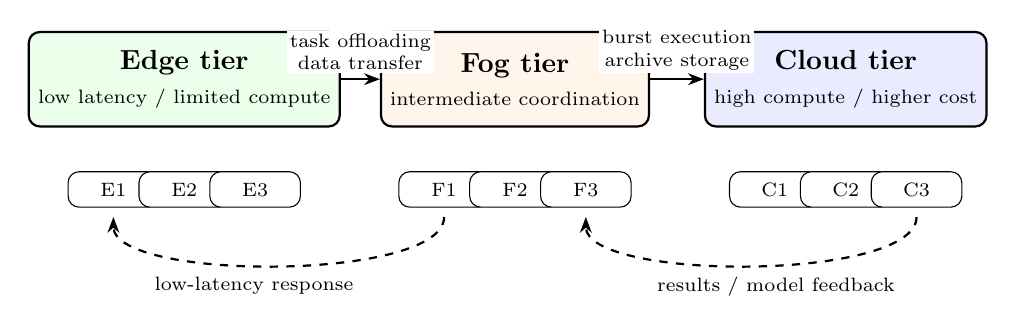
\begin{tikzpicture}[
  tier/.style={draw, rounded corners, thick, minimum width=3.4cm, minimum height=1.2cm, align=center, fill=#1!8},
  nbox/.style={draw, rounded corners, font=\scriptsize, inner sep=2pt, minimum width=1.15cm, minimum height=0.45cm, fill=white},
  link/.style={-{Stealth[length=2mm]}, thick}
]
  % Tier labels (top row)
  \node[tier=green]  (edge)  at (0,0)   {\textbf{Edge tier}\\\scriptsize low latency / limited compute};
  \node[tier=orange] (fog)   at (4.2,0) {\textbf{Fog tier}\\\scriptsize intermediate coordination};
  \node[tier=blue]   (cloud) at (8.4,0) {\textbf{Cloud tier}\\\scriptsize high compute / higher cost};

  % Node boxes (below tiers)
  \node[nbox] at (-0.9,-1.4) {E1};
  \node[nbox] at (0,   -1.4) {E2};
  \node[nbox] at (0.9, -1.4) {E3};

  \node[nbox] at (3.3,-1.4) {F1};
  \node[nbox] at (4.2,-1.4) {F2};
  \node[nbox] at (5.1,-1.4) {F3};

  \node[nbox] at (7.5,-1.4) {C1};
  \node[nbox] at (8.4,-1.4) {C2};
  \node[nbox] at (9.3,-1.4) {C3};

  % Forward arrows (between tiers, above node boxes)
  \draw[link] (edge.east)  -- node[midway, above=2pt, font=\scriptsize, align=center, fill=white, inner sep=1pt] {task offloading\\data transfer} (fog.west);
  \draw[link] (fog.east)   -- node[midway, above=2pt, font=\scriptsize, align=center, fill=white, inner sep=1pt] {burst execution\\archive storage} (cloud.west);

  % Feedback arrows (below node boxes)
  \draw[link, dashed] (9.3,-1.75) to[out=-90,in=-90, looseness=0.5]
    node[pos=0.45, below=3pt, font=\scriptsize, fill=white, inner sep=1pt] {results / model feedback}
    (5.1,-1.75);
  \draw[link, dashed] (3.3,-1.75) to[out=-90,in=-90, looseness=0.5]
    node[pos=0.55, below=3pt, font=\scriptsize, fill=white, inner sep=1pt] {low-latency response}
    (-0.9,-1.75);

\end{tikzpicture}
\caption{Simplified Edge/Fog/Cloud execution architecture used to motivate the scheduling model. The heterogeneous compute, bandwidth, and cost properties across tiers create the many-objective trade-offs optimized by ADARE and the compared baselines.}
\label{fig:edge_fog_cloud_arch}
\end{figure}

Figure~\ref{fig:edge_fog_cloud_arch} clarifies the systems setting: edge nodes favor low-latency execution, fog nodes provide coordination and intermediate capacity, and cloud nodes provide stronger compute at a different cost/bandwidth profile. This heterogeneity is the reason a static operator schedule can become suboptimal during search.

\subsection{Objective Vector}
ADARE and all compared baselines optimize the same four-objective minimization vector:
\begin{equation}
\min \; \mathbf{f}(x) = \left(f_{\mathrm{mk}}(x), f_{\mathrm{lat}}(x), f_{\mathrm{cost}}(x), f_{\mathrm{eng}}(x)\right),
\end{equation}
Let task $i$ be assigned to node $x_i$. Its dependency-ready time $R_i$ is the maximum parent completion time plus, for a cross-node dependency, $D_i/\min(u_{x_j},d_{x_i})$, where $D_i$ is the child task's data-size field and $u,d$ are uplink and downlink capacities. Tasks assigned to one node are serialized, hence $S_i=\max(R_i,A_{x_i})$, where $A_{x_i}$ is node availability. The implemented completion time is
\begin{equation}
C_i=S_i+\frac{I_i}{\rho_{x_i}}+\frac{D_i}{u_{x_i}},
\end{equation}
with instruction count $I_i$ and processing rate $\rho_{x_i}$. The final term is the evaluator's outgoing-data overhead. The four objectives are then
\begin{equation}
\label{eq:objective_metrics}
\begin{aligned}
f_{\mathrm{mk}}(x) &= \max_{i \in V} C_i, \\
f_{\mathrm{lat}}(x) &= \sum_{i \in V} \left(C_i - R_i\right), \\
f_{\mathrm{cost}}(x) &= \sum_{i \in V} \left(\frac{I_i}{\rho_{x_i}}\right) c_{x_i}, \\
f_{\mathrm{eng}}(x) &= \sum_{i \in V} \left(\frac{I_i}{\rho_{x_i}}\right) p^{\mathrm{wrk}}_{x_i}.
\end{aligned}
\end{equation}
Thus latency is aggregate post-readiness residence time, including node queueing, execution, and outgoing overhead. Cost is compute-time charge and energy is a compute-only working-power proxy. Idle and communication energy and transfer charges are not included; the idle-power input is not used by this evaluator. Moreover, the JSON fields are treated as simulator units: absent calibration, the outputs should not be read as measurements from a deployed platform. These boundaries are important when interpreting the resource scenarios.

\subsection{Evaluation Targets and Quality Indicators}
We assess final survival populations with hypervolume (HV), inverted generational distance (IGD), spacing, additive epsilon, and coverage \cite{zitzler2003performance}, complemented by runtime and best objective values. Reference points/fronts are constructed jointly within each matched comparison. Using several indicators avoids attributing convergence, coverage, and distribution quality to one scalar summary.

\section{ADARE Methodology: Learning-Guided Adaptive Control}
\subsection{Design Overview}
ADARE is an adaptive extension of NSGA-III, not a new environmental-selection algorithm. It retains NSGA-III reference-point survival and surrounds it with three control modules: contextual crossover selection, density-aware mutation/local repair, and bounded archive injection. Figure~\ref{fig:adare_structure} summarizes the implementation.

\begin{figure}[t]
\centering
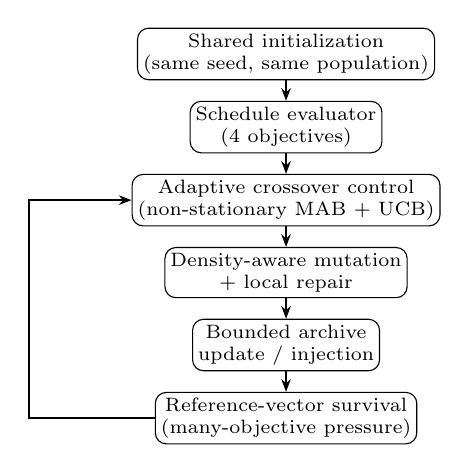
\begin{tikzpicture}[
node distance=2.6mm,
box/.style={draw, rounded corners, align=center, font=\scriptsize, inner sep=2pt},
arr/.style={-{Stealth[length=1.6mm]}, thick}
]
\node[box] (init) {Shared initialization\\(same seed, same population)};
\node[box, below=of init] (eval) {Schedule evaluator\\(4 objectives)};
\node[box, below=of eval] (cross) {Adaptive crossover control\\(non-stationary MAB + UCB)};
\node[box, below=of cross] (mut) {Density-aware mutation\\+ local repair};
\node[box, below=of mut] (arch) {Bounded archive\\update / injection};
\node[box, below=of arch] (sel) {Reference-vector survival\\(many-objective pressure)};
\draw[arr] (init) -- (eval);
\draw[arr] (eval) -- (cross);
\draw[arr] (cross) -- (mut);
\draw[arr] (mut) -- (arch);
\draw[arr] (arch) -- (sel);
\draw[arr] (sel.west) -- ++(-1.6,0) |- (cross.west);
\end{tikzpicture}
\caption{ADARE as a learning-guided workflow scheduler: online search control surrounds a reference-vector environmental selection step.}
\label{fig:adare_structure}
\end{figure}

\subsection{Learning Formalization: Pareto-Contextual MAB for Operator Control}
\label{sec:mab}
The portfolio contains one-point, two-point, and uniform crossover with per-gene exchange probabilities 0.5 and 0.8. Let $s_t=(\rho_t,d_t,z_t)$: phase is early for progress $<0.34$, middle for $[0.34,0.67)$, and late otherwise; diversity is low below 0.45; and stagnation is active when $z/7\geq0.70$, i.e., after five consecutive generations without scalar-score improvement. The diagnostic stagnation score is $0.3\log(1+f_{\rm mk})+0.3\log(1+f_{\rm lat})+0.2\log(1+f_{\rm cost})+0.2\log(1+f_{\rm eng})$; it is not used for environmental survival. The controller therefore has 12 contexts and four actions.

With probability $\epsilon_g$, linearly annealed from 0.30 to 0.05, an action is sampled uniformly. Otherwise ADARE selects
\begin{equation}
\label{eq:ucb}
a_t = \arg\max_k \left( Q_{s_t,k} + \sqrt{\frac{2 \ln (N_{s_t}+2)}{N_{s_t,k} + 1}} \right),
\end{equation}
where $N_{s_t}$ and $N_{s_t,k}$ are context and action counts. All values and counts start at zero; deterministic score ties select the first portfolio entry.

\paragraph{Reward definition.}
Let $P=\{p_1,p_2\}$ and $C=\{c_1,c_2\}$ be parent and evaluated child objective vectors. For each objective $j$, $\Delta_j=(\min_{p\in P}f_j(p)-\min_{c\in C}f_j(c))/s_j$, where $s_j$ is the current population range (with a robust nonzero fallback). ADARE computes
\begin{equation}
\label{eq:reward}
r_t =
0.45D(P,C) + 0.35I(P,C) + 0.15B(P,C) + 0.05V(P,C),
\end{equation}
where $D=(n_{\rm hit}-n_{\rm dominated})/2$, counting children that dominate any parent and children dominated by both parents; $I=\frac14\sum_j\operatorname{clip}(\Delta_j,-1,1)$; $B=\frac14\sum_j\mathbb{1}[\Delta_j>0]$; and $V$ is the mean normalized Hamming distance over the four child--parent pairs. The resulting reward is clipped to $[-1,1]$. It is computed after crossover, mutation, optional repair, archive injection, and objective evaluation, but before NSGA-III survival. The selected value is updated by
\begin{equation}
Q_{s_t,k} \leftarrow (1-\alpha)Q_{s_t,k} + \alpha r_t,\qquad \alpha=0.22.
\end{equation}
The trace exports context, action, reward, diversity, stagnation, and the fraction of both children surviving environmental selection.

\begin{algorithm}[H]
\caption{ADARE Pareto-Contextual UCB Crossover Control}
\label{alg:ucb_control}
\small
\begin{algorithmic}[1]
\Require Parent pair $(p_1,p_2)$, population diversity $d$, stagnation count $z$, phase $\rho$
\State Build context $s \gets (\rho,d,z)$ \Comment{Separate exploration, collapse, and refinement regimes}
\State Select operator index $k$ with $\epsilon$-exploration or Eq.~\eqref{eq:ucb} \Comment{Balance coverage and learned value}
\State Apply crossover, mutation, optional repair/injection, then evaluate $(c_1,c_2)$
\State Compute reward $r_t$ with Eq.~\eqref{eq:reward} \Comment{Credit the complete offspring-producing action}
\State Update $Q_{s,k} \leftarrow (1-\alpha)Q_{s,k} + \alpha r_t$ and $N_{s,k} \leftarrow N_{s,k} + 1$
\State Export $(s,k,r_t,d,z)$ to the controller trace \Comment{Enable post-survival audit}
\State \Return $(c_1,c_2)$
\end{algorithmic}
\end{algorithm}

\subsection{Density-Aware Mutation and Local Repair}
For progress $\rho$, diversity $d$, and $|V|$ genes, the uncapped mutation budget is
\begin{equation}
B=\max\{1,\lfloor[0.01+0.08(1-\rho)+0.10(1-d)]|V|\rfloor\}.
\end{equation}
The experimental configuration caps it at one assignment per triggered individual. With probability 0.55, that assignment samples among the three highest-ranked nodes; otherwise it is random. The node score is $q_i\hat\rho+(1-q_i)\hat u-0.12\hat c-0.11\hat p$, with $q_i=I_i/(I_i+10^5D_i)$ and min--max-normalized node attributes. A subsequent gene pass uses probability $0.08[0.20+0.30(1-d)]$ per gene.

\begin{algorithm}[H]
\caption{Density-Aware Mutation with Heuristic Guidance}
\label{alg:density_mutation}
\small
\begin{algorithmic}[1]
\Require Individual $x$, diversity score $d$, generation $g$, task-node rankings $\mathcal{R}$
\State Compute and cap mutation budget $B$ \Comment{Raise pressure as progress/diversity fall}
\For{$b = 1$ to $B$}
    \State Sample a task index $i$
    \State Set $x_i$ using heuristic-ranked nodes or a random fallback
\EndFor
\State Apply a low-probability gene-level mutation pass \Comment{Retain distributed exploration}
\State With probability $0.05[0.20+0.80(1-d)][0.50+0.50\min(1,z/7)]$, repair a mutated child \Comment{Spend local search under collapse/stagnation}
\State \Return mutated individual $x$
\end{algorithmic}
\end{algorithm}

Local repair tests the two highest-priority tasks and their two best-ranked nodes and accepts a candidate if it dominates the incumbent or improves the diagnostic log score. The archive is bounded at 80 schedules, updated every six generations, and injected at rate 0.02. Crucially, every reported comparative metric---including best-objective values---uses only the equally sized final NSGA-III survival population. Archive or hand-built candidates are never appended to the scored set.

\subsection{Complexity and Measured Control Overhead}
The schedule evaluator dominates runtime. For population size $P$, generation count $G$, task count $|V|$, and average dependency-processing factor $\bar d$, evaluation cost is approximately
\begin{equation}
\mathcal{O}(G \cdot P \cdot |V| \cdot \bar d).
\end{equation}
The four-action controller is constant-time per mating and its table is $12\times4$. Mutation and schedule evaluation scale with $|V|$; NSGA-III survival retains its usual population-dependent cost. Instrumented results below separate selection, reward/update, archive, evaluation, and survival rather than inferring overhead from total runtime.

\section{Experimental Protocol and Results}
\subsection{Artifact, platform, and protocol}
All experiments use Python 3.13.1 on an ASUS TUF Gaming A15 with an AMD Ryzen 5 7535HS (12 logical CPUs), 16~GB RAM, and Windows 11. Objective evaluation uses ten CPU worker processes when the batch is large enough; the evolutionary control itself remains CPU-based. The installed RTX 2050 is not used because the evaluator and evolutionary operators are branch-heavy Python/NumPy workloads rather than GPU kernels.

The nominal environment has five nodes per tier and follows the artifact's Edge--Fog--Cloud template \cite{mohan2016edgefog}. Edge, fog, and cloud processing rates are 1000, 1300, and 1600; processing costs are 0.02, 0.48, and 0.96; working powers are 700, 700, and 1648; and uplink/downlink capacities are 20480/20480, 10000/10000, and 100/10000, respectively. These are simulator parameters in the units supplied by the artifact. The small suite uses Montage\_25, CyberShake\_30, and Epigenomics\_24. Large suites use four 1000-task Pegasus instances and five WfCommons-generated instances in the 3000-task class; one diagnostic Montage instance contains 2991 parsed tasks.

Within every matched run, algorithms receive the same seed, initial population, evaluator, population size, and generation count. The protocols are: small, 20 runs, $P=100$, $G=70$; 1000-task, 20 runs, $P=80$, $G=50$ and 100; 3000-task class, 10 runs, $P=60$, $G=20$; and scaling/resource diagnostics, 10 runs, $P=60$, $G=30$. Fitness caching means duplicate schedules need not be re-evaluated, so generation/population budgets are matched while realized unique objective-evaluation counts may differ. We report those counts and plot convergence against both evaluations and wall time.

The baselines are NSGA-II, MOEA/D, NSGA-III, QL-NSGA-III, and workflow adaptations inspired by OVEA and QMOEA/D-AWA. The latter two are not claimed as exact reproductions of the published artifacts. Each final comparison uses the non-dominated subset of the equally sized survival population. For every benchmark--baseline--indicator pair we apply a paired one-sided Wilcoxon signed-rank test \cite{wilcoxon1945} in the favorable ADARE direction, Holm-correct the resulting family, report paired rank-biserial effect size, and calculate a deterministic paired-bootstrap 95\% confidence interval. Zero differences are retained according to the implemented Wilcoxon convention. Direction, multiplicity-adjusted significance, and the interval are interpreted together; an unadjusted $p$-value is not treated as confirmatory evidence by itself.

\subsection{Main paired results}
Table~\ref{tab:protocol-summary} reports favorable paired effects for the five core indicators. It intentionally avoids collapsing dissimilar indicators into one ``overall gain.'' On the small workflows ADARE is favorable in 81/90 comparisons, 48 of which remain Holm-significant. At 1000 tasks, 78/80 comparisons favor ADARE at 50 generations and 69/80 at 100 generations, with 56 and 55 Holm-significant, respectively. The longer budget is an important boundary result: QL-NSGA-III becomes competitive and ADARE is favorable in only 9/20 indicator comparisons against it. At the 3000-task class, 88/100 comparisons favor ADARE, but only 33 are Holm-significant.

\begin{table}[t]
\caption{Directional paired evidence across the confirmatory protocols. A ``win'' means a favorable paired effect, not necessarily statistical significance.}
\label{tab:protocol-summary}
\centering\small
\resizebox{\textwidth}{!}{\begin{tabular}{lrrrr}
\toprule
Protocol & Tests & ADARE wins & Holm-significant wins & Positive 95\% CI \\
\midrule
Small, 70 gen. & 90 & 81 & 48 & 68 \\
1000 tasks, 50 gen. & 80 & 78 & 56 & 56 \\
1000 tasks, 100 gen. & 80 & 69 & 55 & 57 \\
3000-task class, 20 gen. & 100 & 88 & 33 & 63 \\
\bottomrule
\end{tabular}
}
\end{table}

\begin{table}[t]
\caption{Core-indicator results by adaptive baseline and long-budget protocol.}
\label{tab:long-budget}
\centering\small
\resizebox{\textwidth}{!}{\begin{tabular}{llrr}
\toprule
Protocol & Baseline & ADARE wins & Holm-significant wins \\
\midrule
1000 tasks, 50 gen. & NSGA-III & 19/20 & 16/20 \\
1000 tasks, 50 gen. & OVEA-style & 20/20 & 20/20 \\
1000 tasks, 50 gen. & QL-NSGA-III & 19/20 & 0/20 \\
1000 tasks, 50 gen. & QMOEA/D-AWA-style & 20/20 & 20/20 \\
1000 tasks, 100 gen. & NSGA-III & 20/20 & 14/20 \\
1000 tasks, 100 gen. & OVEA-style & 20/20 & 20/20 \\
1000 tasks, 100 gen. & QL-NSGA-III & 9/20 & 1/20 \\
1000 tasks, 100 gen. & QMOEA/D-AWA-style & 20/20 & 20/20 \\
3000-task class, 20 gen. & NSGA-III & 23/25 & 7/25 \\
3000-task class, 20 gen. & OVEA-style & 25/25 & 16/25 \\
3000-task class, 20 gen. & QL-NSGA-III & 18/25 & 0/25 \\
3000-task class, 20 gen. & QMOEA/D-AWA-style & 22/25 & 10/25 \\
\bottomrule
\end{tabular}
}
\end{table}

These results support competitiveness across the tested workflows, not universal dominance. In particular, the 100-generation QL-NSGA-III result shows that conclusions from a short budget can reverse for a strong adaptive baseline.

\subsection{Ablations, sensitivity, and controller validity}
The incremental V1--V5 ablation starts with NSGA-III (V1), then adds UCB crossover control (V2), density-aware mutation (V3), partial archive guidance (V4), and the complete configuration (V5). Relative to V1, V5 has favorable mean core-indicator gain on all three small benchmarks and wins 12/15 individual indicator comparisons. The progression is not monotone indicator by indicator, and every adaptive variant is slower in this isolated runner; V5's mean runtime change is $-10.17\%$. Thus no module is presented as independently sufficient.

\begin{table}[t]
\caption{Incremental V1--V5 ablation (20 paired runs per benchmark). Gains are means relative to V1; positive runtime gain means faster.}
\label{tab:ablation}
\centering\small
\begin{tabular}{lrrrr}
\toprule
Variant & Core gain (\%) & Objective gain (\%) & Runtime gain (\%) & Core wins \\
\midrule
V2 & 3.51 & 6.19 & -11.42 & 11/15 \\
V3 & 3.95 & 6.49 & -9.47 & 10/15 \\
V4 & 4.74 & 6.46 & -9.39 & 9/15 \\
V5 & 6.22 & 6.47 & -10.17 & 12/15 \\
\bottomrule
\end{tabular}
\end{table}

A second controlled ablation holds mutation, archive, survival, evaluator, and budgets fixed while replacing full ADARE with static two-point, global dominance-reward UCB, or contextual dominance-reward UCB. Across 15 comparisons per variant, no result remains significant after Holm correction (Table~\ref{tab:controller-ablation}). This prevents attributing the entire gain to contextual action selection alone; the evidence is more consistent with an interacting controller--reward--variation system.

\begin{table}[t]
\caption{Controlled controller/reward ablation (three workflows, five indicators).}
\label{tab:controller-ablation}
\centering\small
\begin{tabular}{lrrr}
\toprule
Comparator/variant & ADARE wins & Raw $p<0.05$ & Holm $p<0.05$ \\
\midrule
Contextual-UCB & 11/15 & 1 & 0 \\
Global-UCB & 11/15 & 0 & 0 \\
Static & 8/15 & 2 & 0 \\
\bottomrule
\end{tabular}

\end{table}

Reward-weight, learning-rate, and clipping perturbations likewise produce no Holm-significant differences from the default across 105 comparisons. Disabling clipping is exactly identical to the default in these runs, showing that the default bound never activates. The result is evidence of local robustness, not proof that the reward parameters are optimal.

\begin{table}[t]
\caption{Reward sensitivity relative to default ADARE.}
\label{tab:reward-sensitivity}
\centering\small
\begin{tabular}{lrrr}
\toprule
Comparator/variant & ADARE wins & Raw $p<0.05$ & Holm $p<0.05$ \\
\midrule
Dominance-heavy & 12/15 & 3 & 0 \\
Equal-weights & 9/15 & 1 & 0 \\
High-alpha & 11/15 & 3 & 0 \\
Improvement-heavy & 10/15 & 0 & 0 \\
Low-alpha & 8/15 & 1 & 0 \\
No-clipping & 0/15 & 0 & 0 \\
Tight-clipping & 10/15 & 2 & 0 \\
\bottomrule
\end{tabular}

\end{table}

Controller traces provide a downstream validity check independent of final front quality. Immediate reward is positively associated with the fraction of both children surviving NSGA-III selection in every one of 20 runs on each 1000-task workflow (Table~\ref{tab:reward-survival}). Inference is performed on the 20 run-level Spearman correlations, not on pooled mating events. Operator use is distributed across the portfolio; one- and two-point crossover account for roughly 25--27\% each and uniform-0.5 roughly 22\%, with modest context-dependent shifts (Fig.~\ref{fig:controller-behavior}).

\begin{table}[t]
\caption{Run-level association between immediate controller reward and offspring survival.}
\label{tab:reward-survival}
\centering\small
\resizebox{\textwidth}{!}{\begin{tabular}{lrrrrr}
\toprule
Benchmark & Runs & Mean $\rho$ & 95\% CI & One-sided $p$ & Positive runs \\
\midrule
CyberShake\_1000 & 20 & 0.324 & [0.311, 0.337] & 9.54e-07 & 20/20 \\
Montage\_1000 & 20 & 0.265 & [0.256, 0.273] & 9.54e-07 & 20/20 \\
\bottomrule
\end{tabular}
}
\end{table}

\begin{figure}[t]
\centering
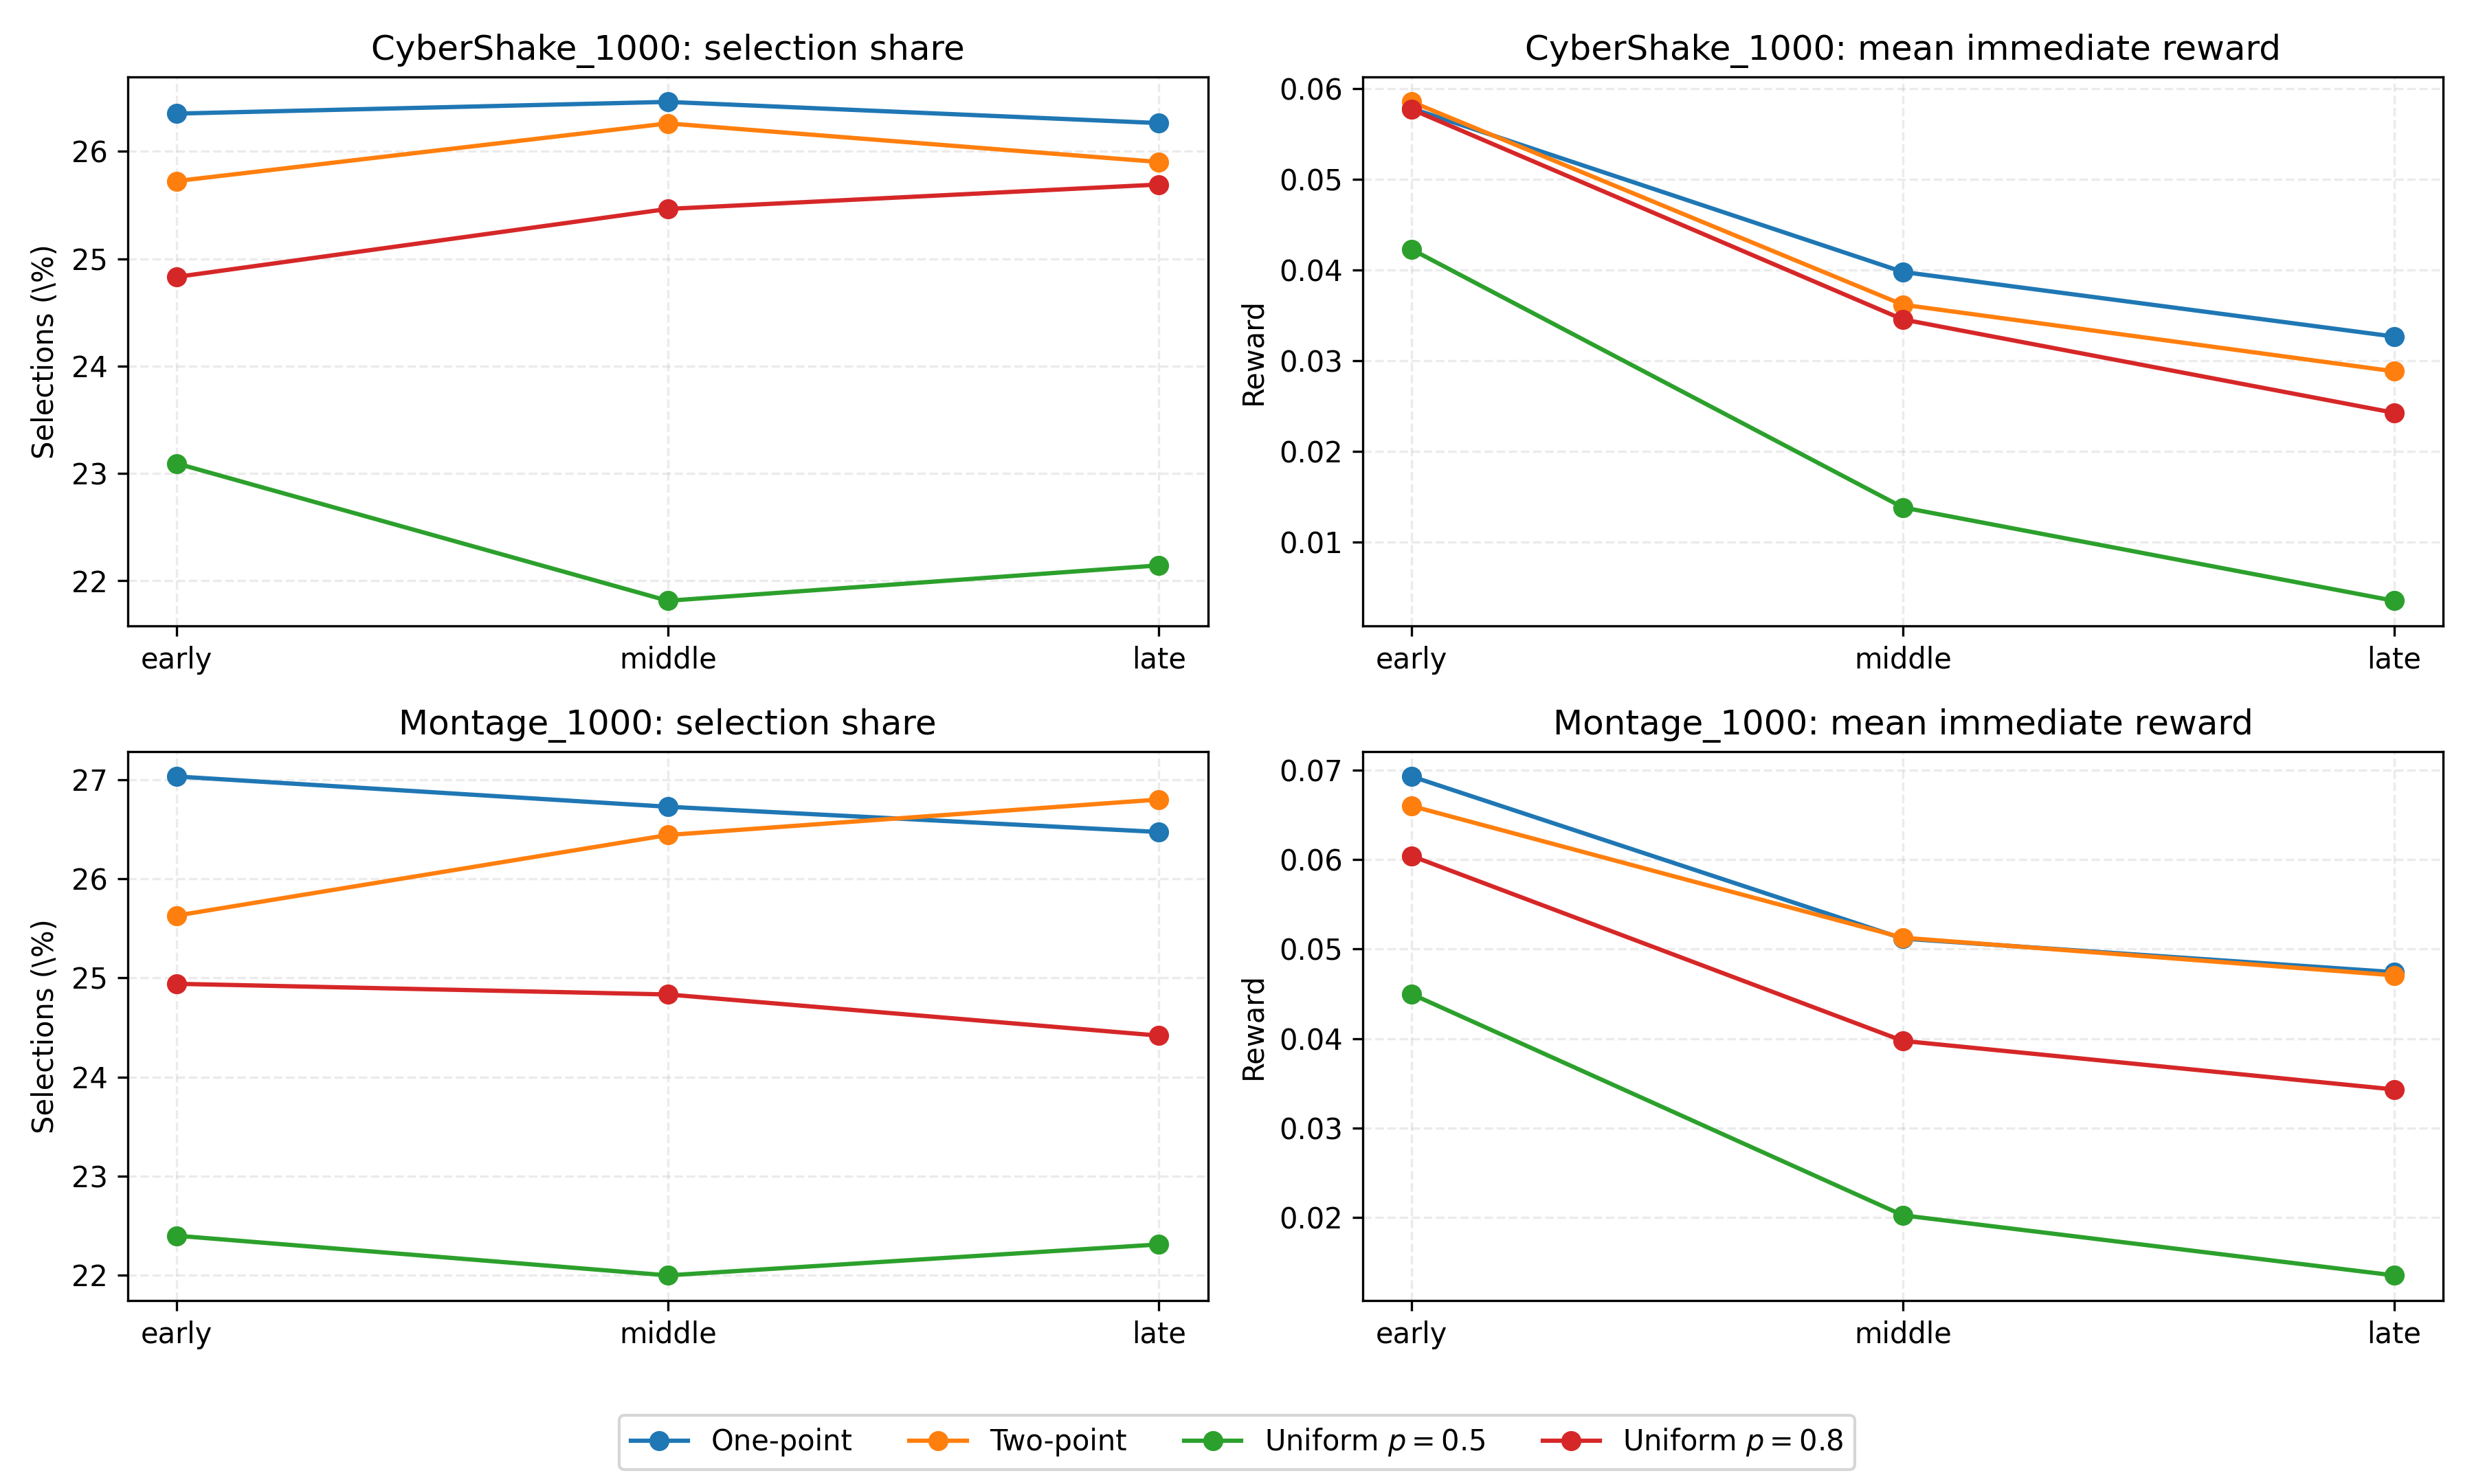
\includegraphics[width=0.92\textwidth]{revision_controller_behavior.png}
\caption{Controller use and reward by phase/operator. Error bars summarize run-level uncertainty.}
\label{fig:controller-behavior}
\end{figure}

\subsection{Convergence, overhead, and resource diagnostics}
Figures~\ref{fig:conv-evals} and~\ref{fig:conv-time} show the same runs against realized objective evaluations and elapsed time. This dual view is necessary because the cache makes unique-evaluation trajectories algorithm-dependent.

\begin{figure}[t]
\centering
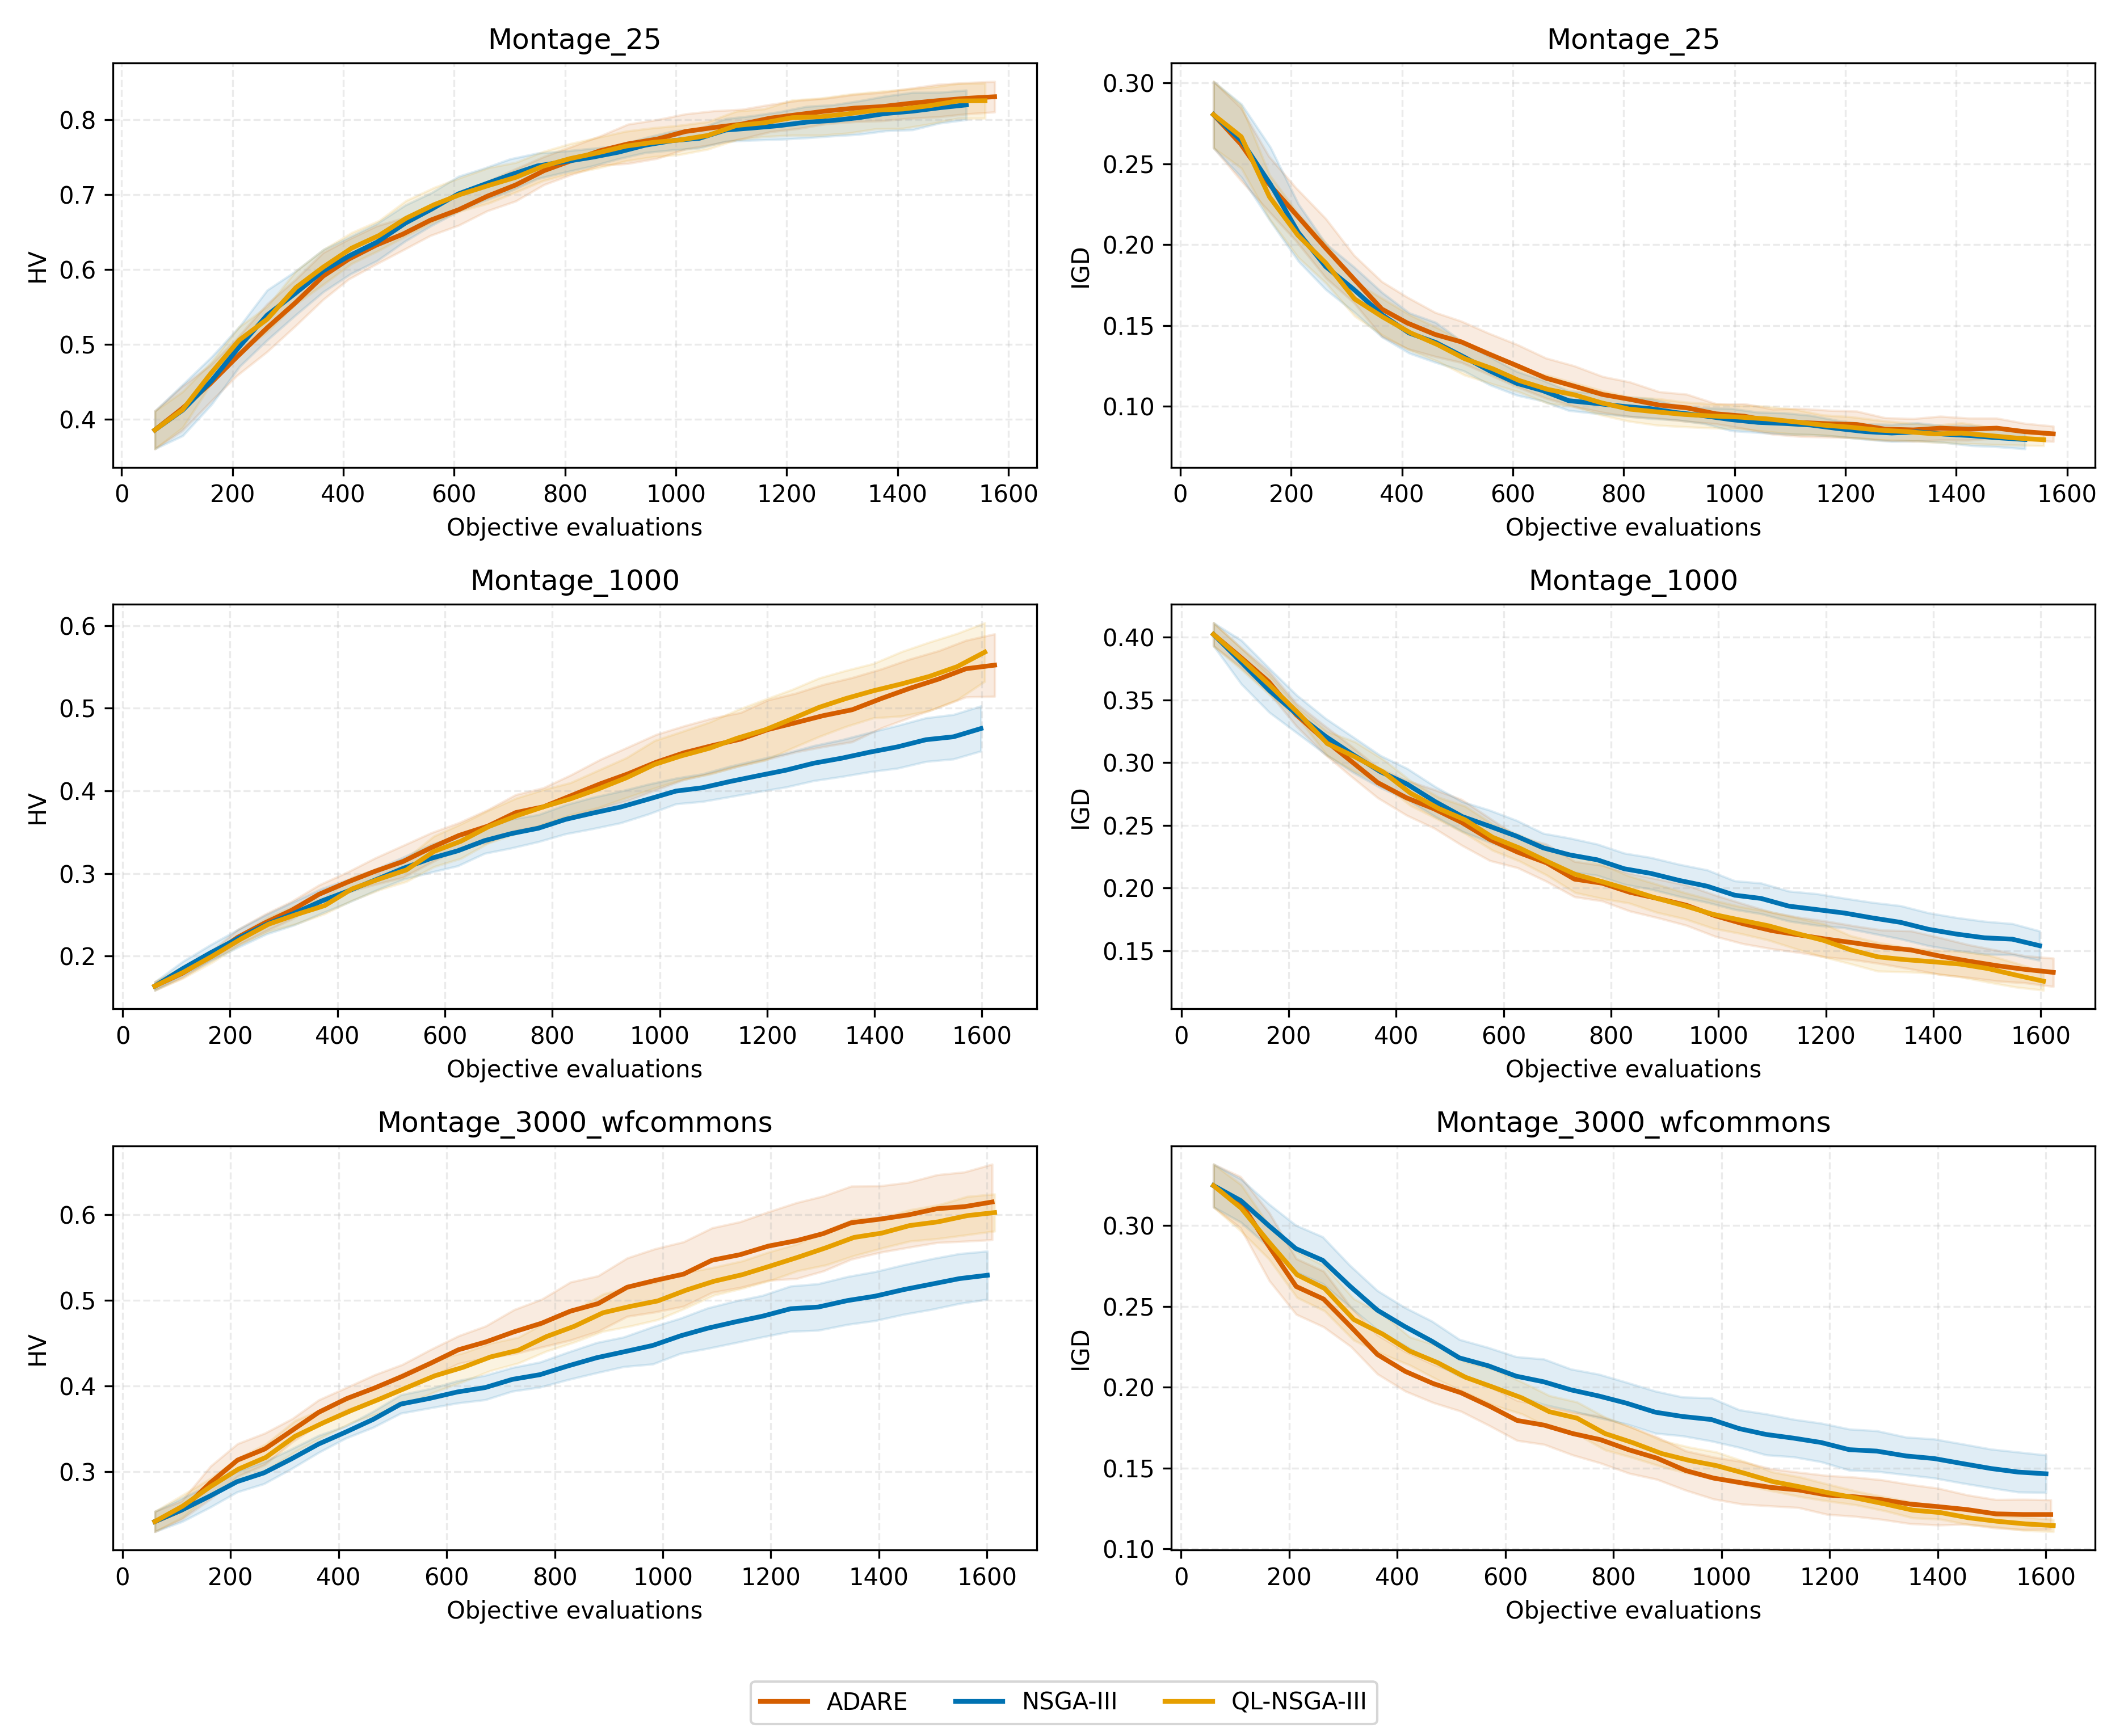
\includegraphics[width=0.96\textwidth]{revision_convergence_vs_evaluations.png}
\caption{Mean convergence trajectories against realized objective evaluations; bands are 95\% confidence intervals across runs.}
\label{fig:conv-evals}
\end{figure}

\begin{figure}[t]
\centering
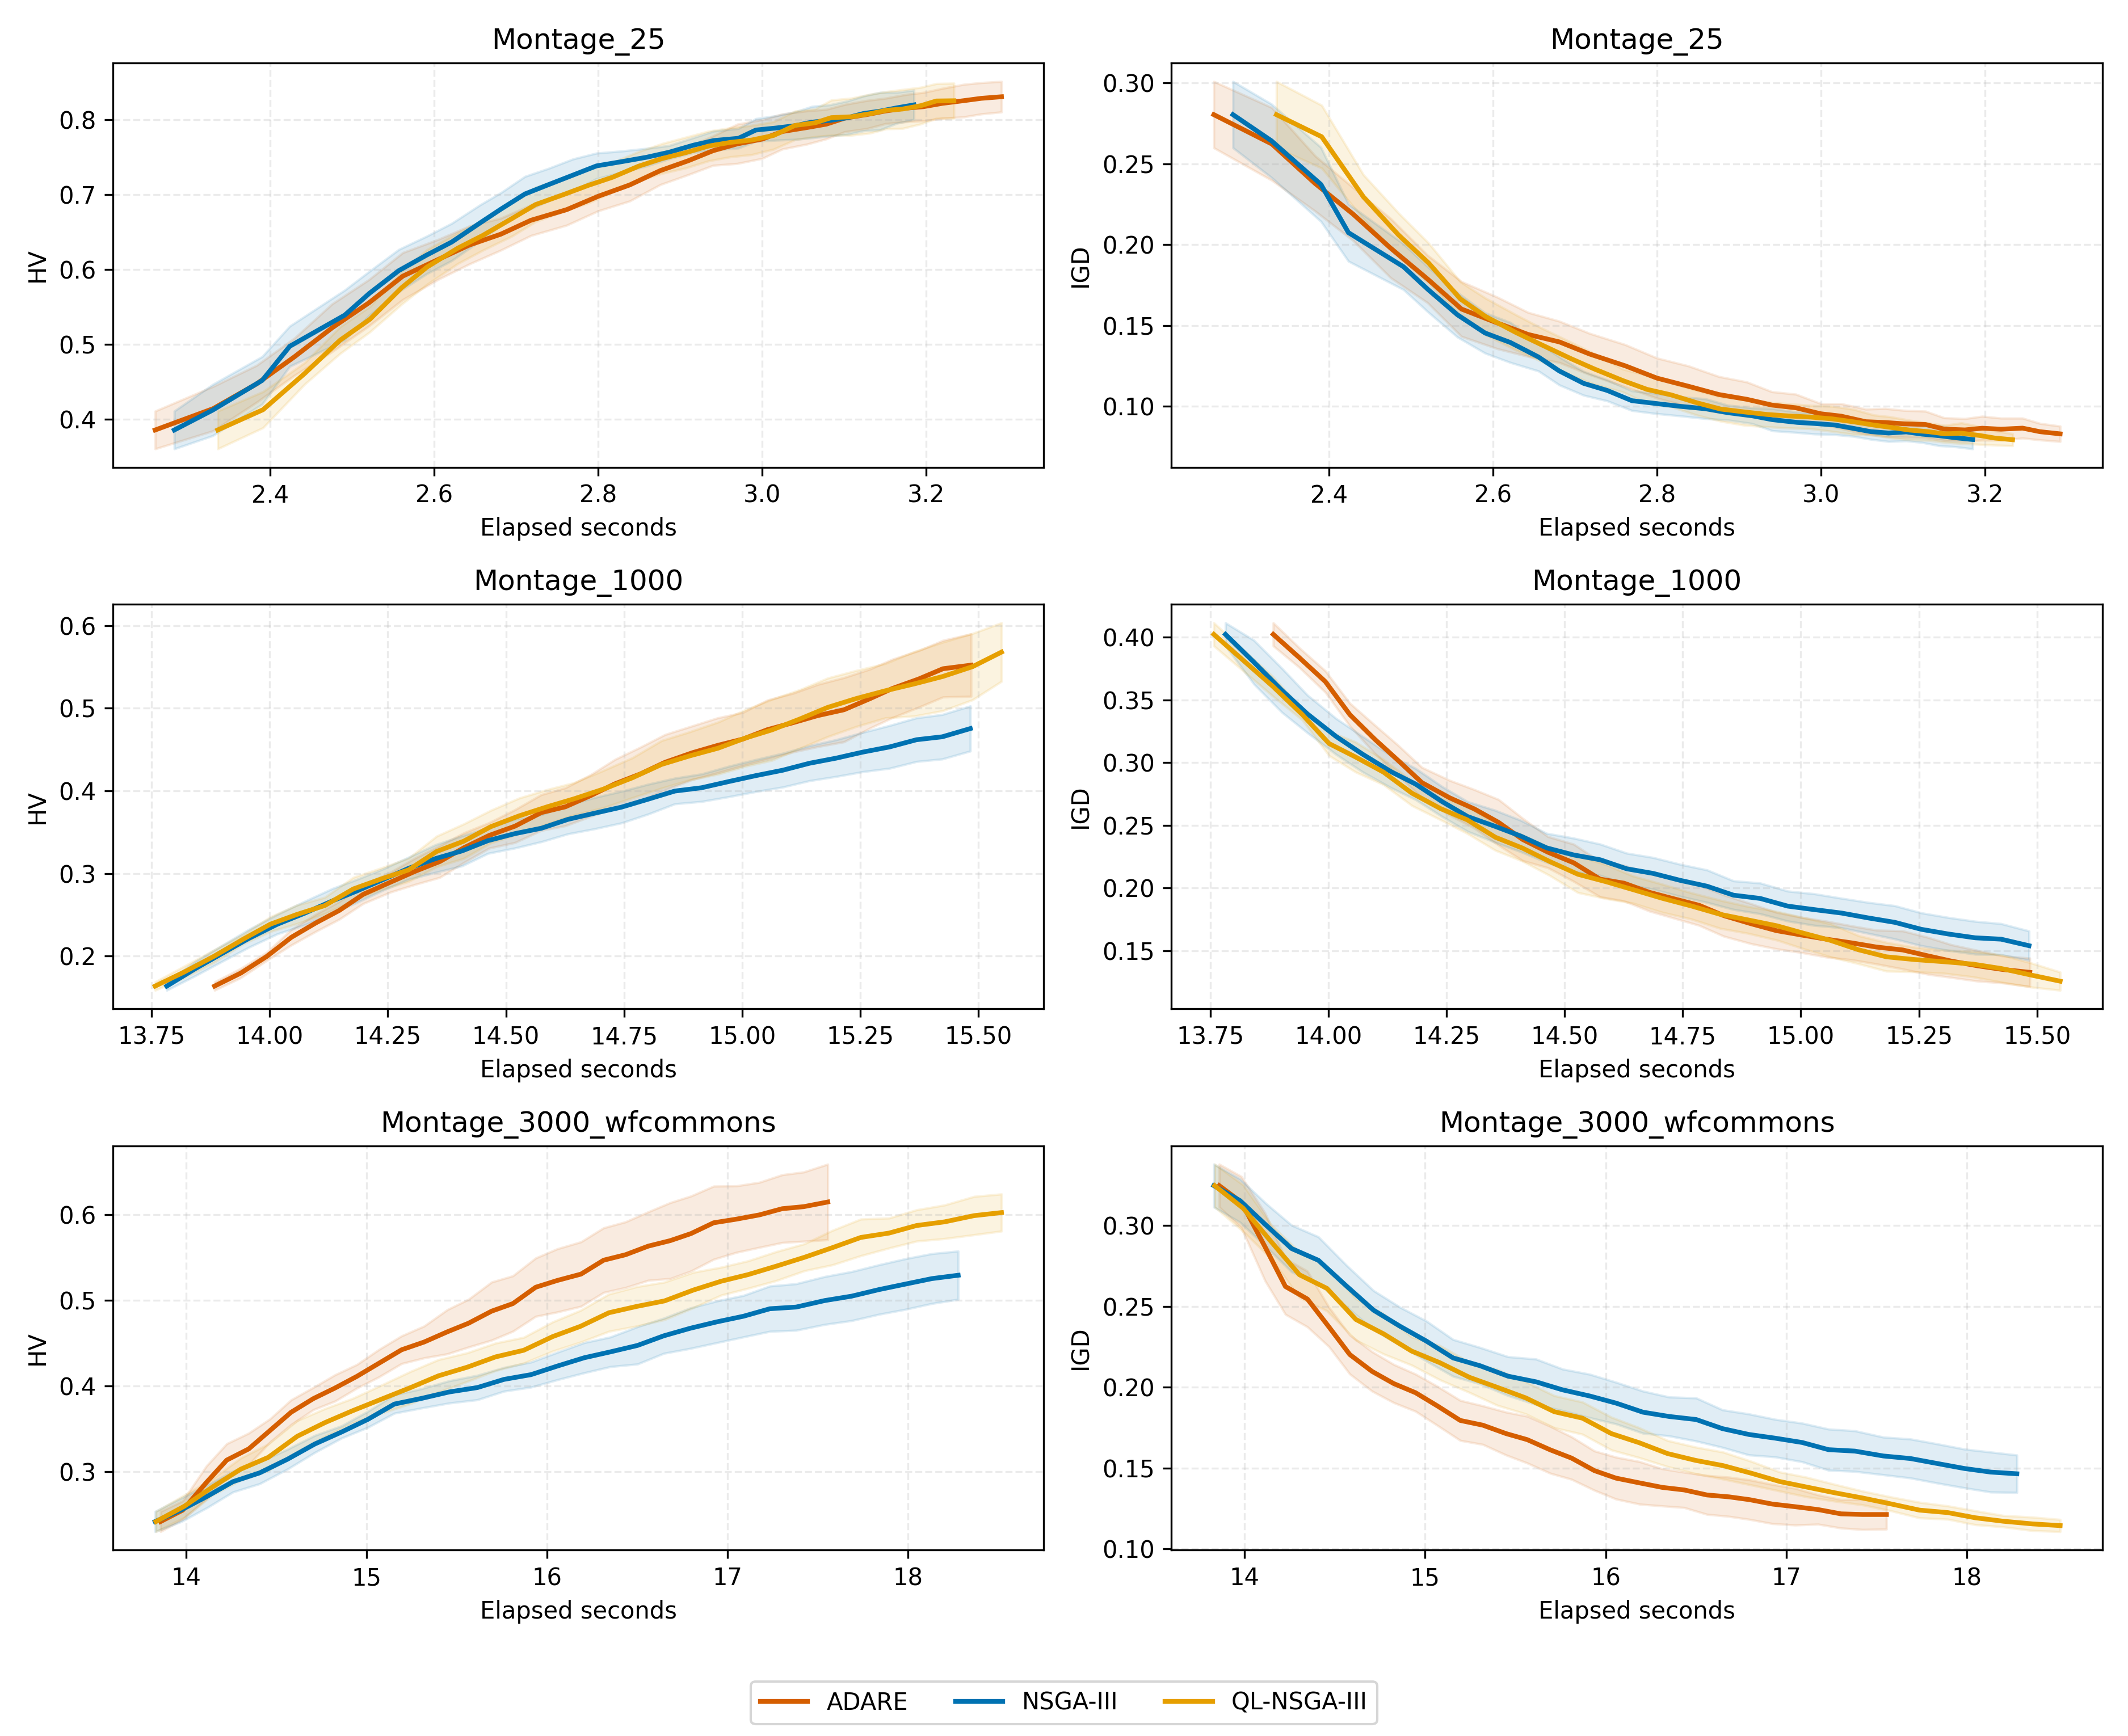
\includegraphics[width=0.96\textwidth]{revision_convergence_vs_time.png}
\caption{The same diagnostic trajectories against wall-clock time, with 95\% confidence intervals.}
\label{fig:conv-time}
\end{figure}

Direct instrumentation on the 1000-task, 100-generation traces assigns about 0.27\% of total runtime to controller selection and 4.8\% to reward calculation and value update; archive operations account for about 0.25\%. Initialization dominates the recorded wall time (about 71--72\%), while fitness evaluation inside the generational loop accounts for about 14--15\%. These shares are implementation- and hardware-specific.

\begin{table}[t]
\caption{Measured ADARE runtime components on the final 1000-task trace protocol.}
\label{tab:runtime-breakdown}
\centering\small
\resizebox{\textwidth}{!}{\begin{tabular}{llrr}
\toprule
Benchmark & Component & Mean seconds & Share of runtime \\
\midrule
CyberShake\_1000 & archive\_operations & 0.046 & 0.25\% \\
CyberShake\_1000 & controller\_selection & 0.052 & 0.28\% \\
CyberShake\_1000 & fitness\_evaluation & 2.658 & 14.25\% \\
CyberShake\_1000 & reward\_and\_controller\_update & 0.912 & 4.89\% \\
Montage\_1000 & archive\_operations & 0.047 & 0.25\% \\
Montage\_1000 & controller\_selection & 0.052 & 0.27\% \\
Montage\_1000 & fitness\_evaluation & 2.885 & 15.27\% \\
Montage\_1000 & reward\_and\_controller\_update & 0.911 & 4.82\% \\
\bottomrule
\end{tabular}
}
\end{table}

Process-tree memory is sampled every 0.05~s while ten evaluator workers are active. Incremental peak resident memory rises from approximately 1.23~GiB at 25 tasks to 1.28~GiB at 2991 tasks and differs little among methods (Table~\ref{tab:runtime-memory}). These are process-tree peaks above the pre-run baseline, not per-process allocations. The short 30-generation diagnostic also finds ADARE about 3.9\% faster than NSGA-III and 5.2\% faster than QL-NSGA-III at 2991 tasks, but no general asymptotic claim follows from three observed sizes.

\begin{table}[t]
\caption{Runtime and sampled process-tree memory scaling (mean $\pm$ 95\% confidence interval).}
\label{tab:runtime-memory}
\centering\small
\begin{tabular}{rlrr}
\toprule
Tasks & Algorithm & Time (s) & Incremental peak RSS (MiB) \\
\midrule
25 & ADARE & 3.29 $\pm$ 0.16 & 1228.6 $\pm$ 1.3 \\
25 & NSGA-III & 3.18 $\pm$ 0.10 & 1227.4 $\pm$ 1.3 \\
25 & QL-NSGA-III & 3.23 $\pm$ 0.16 & 1227.9 $\pm$ 1.2 \\
1000 & ADARE & 15.49 $\pm$ 0.17 & 1246.5 $\pm$ 3.3 \\
1000 & NSGA-III & 15.48 $\pm$ 0.12 & 1242.8 $\pm$ 2.1 \\
1000 & QL-NSGA-III & 15.55 $\pm$ 0.05 & 1242.9 $\pm$ 1.7 \\
2991 & ADARE & 17.56 $\pm$ 0.06 & 1278.4 $\pm$ 11.7 \\
2991 & NSGA-III & 18.28 $\pm$ 0.16 & 1282.2 $\pm$ 7.8 \\
2991 & QL-NSGA-III & 18.52 $\pm$ 0.09 & 1280.3 $\pm$ 8.2 \\
\bottomrule
\end{tabular}

\end{table}

Resource perturbations use Montage\_1000 with nominal resources, compute skew (Edge processing rate $\times0.65$, Cloud $\times1.50$), and network scarcity (all bandwidths $\times0.25$). ADARE is robust under network scarcity, winning 4/5 indicators against NSGA-III (all four Holm-significant) and 5/5 against QL-NSGA-III (none Holm-significant). Under compute skew it wins only 2/5 and 1/5, respectively. Table~\ref{tab:resource} and Fig.~\ref{fig:resource} therefore delimit rather than erase configuration sensitivity.

\begin{table}[t]
\caption{Resource-sensitivity results on Montage\_1000.}
\label{tab:resource}
\centering\small
\resizebox{\textwidth}{!}{\begin{tabular}{llrr}
\toprule
Resource scenario & Algorithm & HV (mean $\pm$ 95\% CI) & IGD (mean $\pm$ 95\% CI) \\
\midrule
nominal & ADARE & 0.552 $\pm$ 0.038 & 0.133 $\pm$ 0.011 \\
nominal & NSGA-III & 0.475 $\pm$ 0.027 & 0.154 $\pm$ 0.012 \\
nominal & QL-NSGA-III & 0.568 $\pm$ 0.035 & 0.126 $\pm$ 0.007 \\
compute\_skew & ADARE & 0.590 $\pm$ 0.012 & 0.102 $\pm$ 0.011 \\
compute\_skew & NSGA-III & 0.566 $\pm$ 0.019 & 0.093 $\pm$ 0.003 \\
compute\_skew & QL-NSGA-III & 0.592 $\pm$ 0.012 & 0.092 $\pm$ 0.004 \\
network\_scarce & ADARE & 0.572 $\pm$ 0.021 & 0.130 $\pm$ 0.005 \\
network\_scarce & NSGA-III & 0.490 $\pm$ 0.030 & 0.153 $\pm$ 0.010 \\
network\_scarce & QL-NSGA-III & 0.549 $\pm$ 0.037 & 0.133 $\pm$ 0.012 \\
\bottomrule
\end{tabular}
}
\end{table}

\begin{figure}[t]
\centering
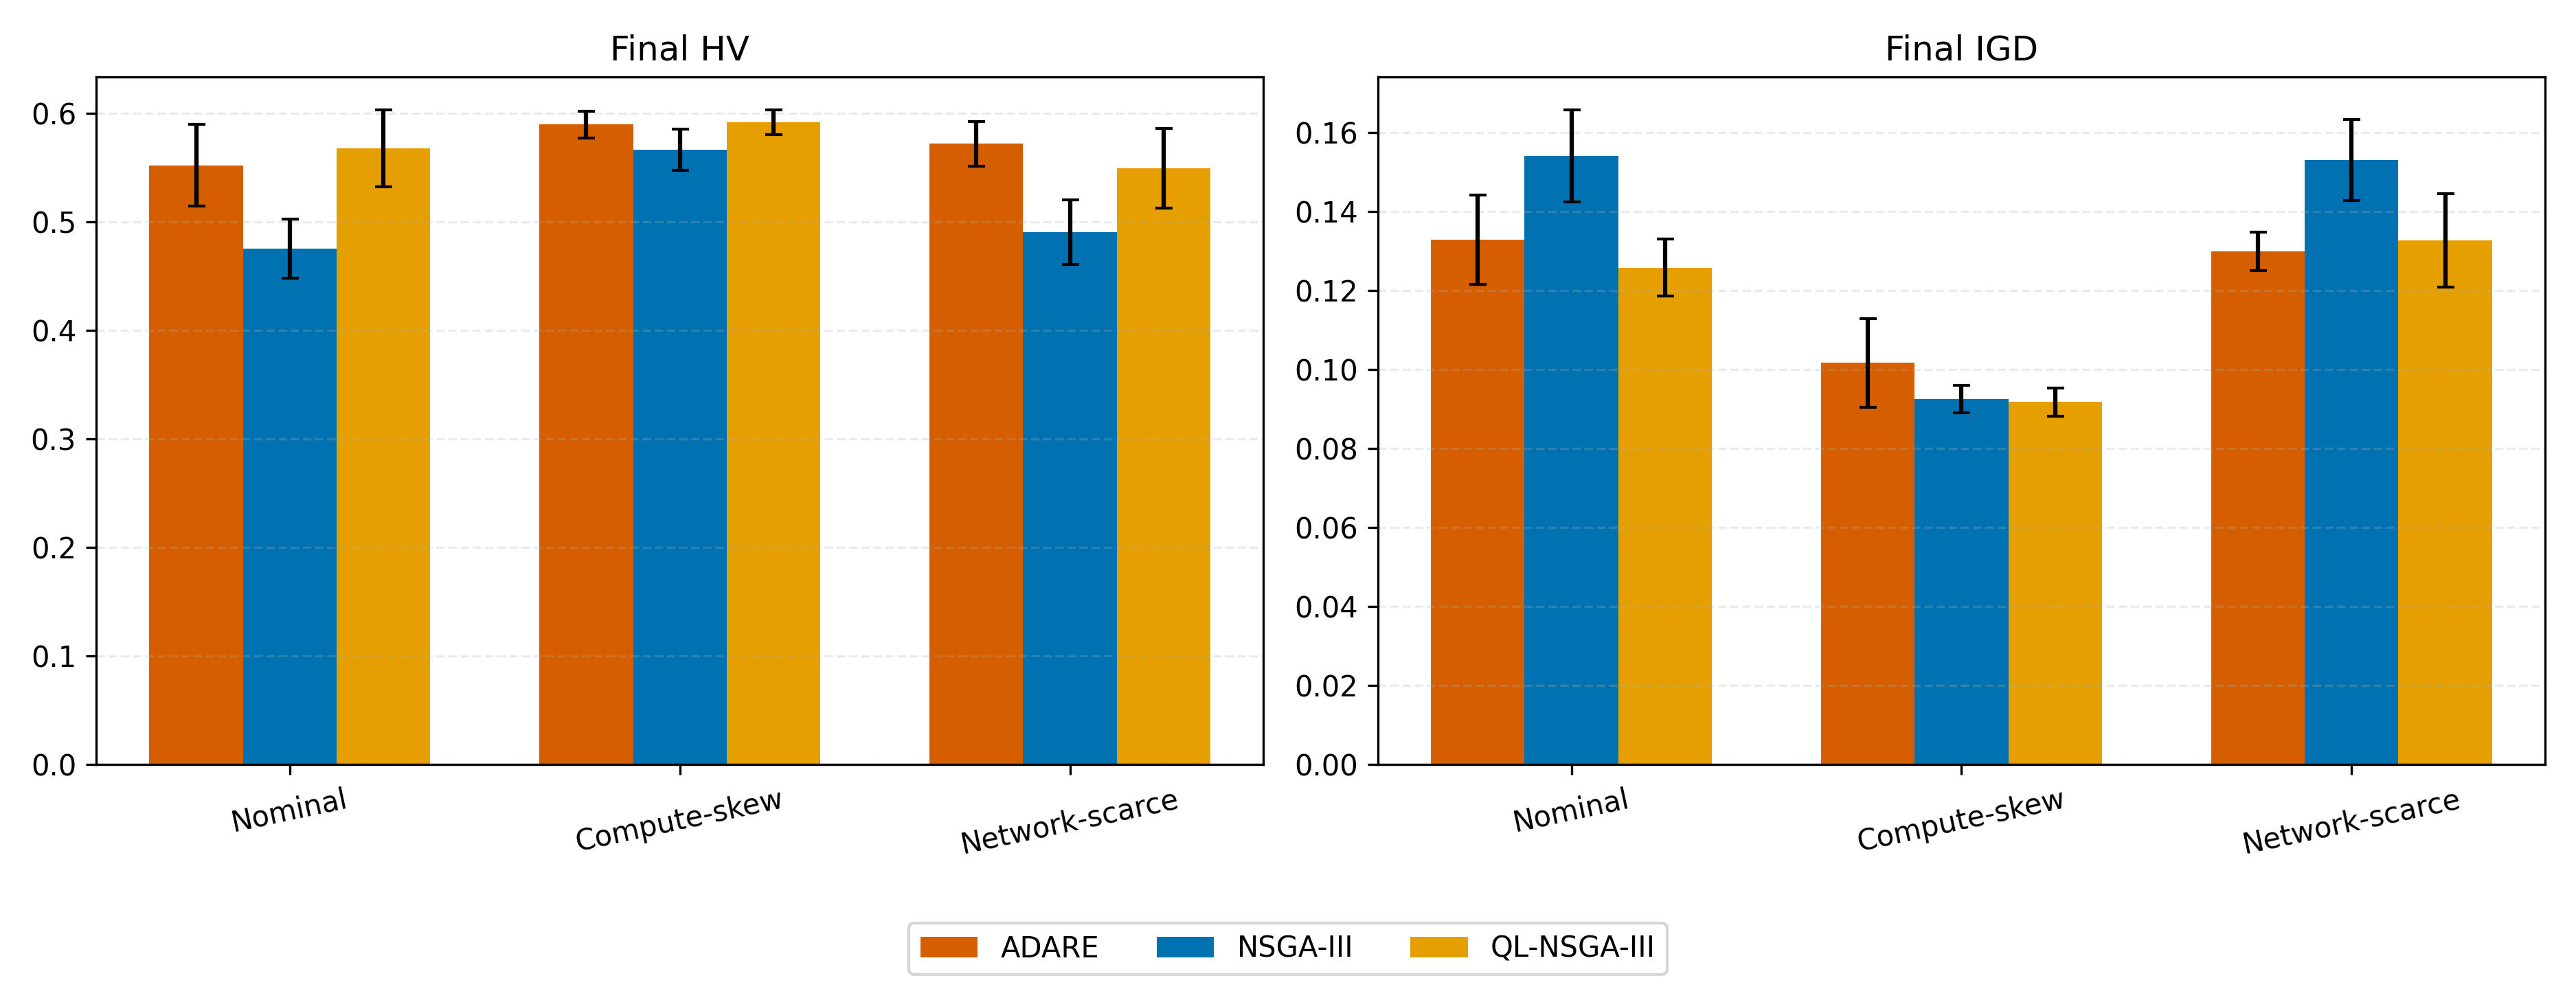
\includegraphics[width=0.92\textwidth]{revision_resource_sensitivity.png}
\caption{HV and IGD under nominal, compute-skewed, and network-scarce configurations (95\% confidence intervals).}
\label{fig:resource}
\end{figure}

\subsection{Objective dependence}
Run-level correlations on the final ADARE fronts confirm genuine trade-offs but also expose partial redundancy (Table~\ref{tab:objective-correlations}). Cost and energy are strongly positively correlated, especially on CyberShake\_1000 (median $\rho=0.93$), because both are compute-time-weighted node attributes in the present evaluator. They are retained because cost and working power rank node types differently, but claims of four independent physical phenomena would be unwarranted.

\begin{table}[t]
\caption{Within-front Spearman correlations, summarized across 20 runs.}
\label{tab:objective-correlations}
\centering\scriptsize
\begin{tabular}{llrr}
\toprule
Benchmark & Objective pair & Median $\rho$ & IQR \\
\midrule
CyberShake\_1000 & cost--energy & 0.93 & [0.92, 0.94] \\
CyberShake\_1000 & latency--cost & -0.72 & [-0.77, -0.66] \\
CyberShake\_1000 & latency--energy & -0.73 & [-0.79, -0.67] \\
CyberShake\_1000 & makespan--cost & -0.89 & [-0.91, -0.89] \\
CyberShake\_1000 & makespan--energy & -0.85 & [-0.88, -0.81] \\
CyberShake\_1000 & makespan--latency & 0.49 & [0.38, 0.59] \\
Montage\_1000 & cost--energy & 0.78 & [0.74, 0.82] \\
Montage\_1000 & latency--cost & -0.42 & [-0.50, -0.31] \\
Montage\_1000 & latency--energy & -0.56 & [-0.61, -0.49] \\
Montage\_1000 & makespan--cost & -0.85 & [-0.88, -0.83] \\
Montage\_1000 & makespan--energy & -0.59 & [-0.66, -0.52] \\
Montage\_1000 & makespan--latency & 0.06 & [-0.05, 0.14] \\
\bottomrule
\end{tabular}

\end{table}

\section{Discussion}
The strongest evidence is the broad paired advantage over classical and adapted baselines under matched initialization, together with positive reward--survival association and low measured selection overhead. The 100-generation and compute-skew results are equally informative: QL-NSGA-III can match or exceed ADARE, and the controlled controller ablation has no Holm-significant advantage. ADARE should therefore be interpreted as a transparent, workflow-tailored adaptive layer whose modules interact, not as an algorithm that dominates every domain or budget.

The study has five principal limitations. First, the deterministic simulator omits failures, contention, idle/communication energy, and transfer charges. Second, cache hits create unequal realized evaluation counts despite equal generation/population budgets; both counts and time are consequently reported. Third, OVEA-style and QMOEA/D-AWA-style are adaptations rather than exact author implementations, while MRL-MOEA and DRLMMEA are discussed but not executed. Fourth, the 3000-task and resource diagnostics use 10 runs and moderate generation budgets. Fifth, one workstation and three resource scenarios cannot establish hardware-independent scalability. Exact public-artifact comparisons, calibrated system traces, multiobjective HEFT variants, and deeper large-scale budgets remain future work.

\section{Conclusion}
ADARE adds an auditable contextual crossover controller, density-aware variation, local repair, and bounded archive guidance to unchanged NSGA-III environmental survival. Across the principal protocols it yields favorable paired effects in 81/90 small-workflow comparisons, 78/80 and 69/80 1000-task comparisons, and 88/100 comparisons in the 3000-task class. Immediate reward predicts offspring survival, while controller selection itself uses roughly 0.27\% of measured runtime. However, strong QL-NSGA-III results at 100 generations, weak isolated-controller significance, and compute-skew sensitivity rule out a universal-superiority claim. The defensible conclusion is that ADARE is a competitive and interpretable adaptive NSGA-III extension for the evaluated deterministic Edge/Fog/Cloud workflow model.

\section*{Declaration of competing interest}
The authors declare that they have no known competing financial interests or personal relationships that could have appeared to influence the work reported in this paper.

\section*{Funding}
This research did not receive any specific grant from funding agencies in the public, commercial, or not-for-profit sectors.

\section*{Data and code availability}
The implementation, experiment scripts, reproduction guide, and generated result artifacts are available at \url{https://github.com/rolln7drktayau/ADARE}.

% Author reasoning clarification
\begin{thebibliography}{99}
\footnotesize
\setlength{\itemsep}{0pt}
\setlength{\parskip}{0pt}
\setlength{\parsep}{0pt}
\bibitem{topcuoglu2002heft}
Topcuoglu, H., Hariri, S., Wu, M.-Y.: Performance-effective and low-complexity task scheduling for heterogeneous computing. IEEE Transactions on Parallel and Distributed Systems \textbf{13}(3), 260--274 (2002)

\bibitem{mohan2016edgefog}
Mohan, N., Kangasharju, J.: Edge-Fog Cloud: A Distributed Cloud for Internet of Things Computations. Presented at IEEE CIoT (2016)

\bibitem{deb2002nsga2}
Deb, K., Pratap, A., Agarwal, S., Meyarivan, T.: A fast and elitist multiobjective genetic algorithm: NSGA-II. IEEE Transactions on Evolutionary Computation \textbf{6}(2), 182--197 (2002)

\bibitem{zhang2007moead}
Zhang, Q., Li, H.: MOEA/D: A multiobjective evolutionary algorithm based on decomposition. IEEE Transactions on Evolutionary Computation \textbf{11}(6), 712--731 (2007)

\bibitem{coleman2021wfcommons}
Coleman, T., Babuji, Y., Li, H., et al.: WfCommons: A framework for enabling scientific workflow research and development. Scientific Data \textbf{9}, 220 (2022).

\bibitem{deb2014nsga3}
Deb, K., Jain, H.: An evolutionary many-objective optimization algorithm using reference-point-based nondominated sorting approach, part I: Solving problems with box constraints. IEEE Transactions on Evolutionary Computation \textbf{18}(4), 577--601 (2014)

\bibitem{auer2002ucb}
Auer, P., Cesa-Bianchi, N., Fischer, P.: Finite-time analysis of the multiarmed bandit problem. Machine Learning \textbf{47}, 235--256 (2002)

\bibitem{dacosta2008aos}
Da Costa, L., Fialho, A., Schoenauer, M., Sebag, M.: Adaptive operator selection with dynamic multi-armed bandits. In: GECCO, pp.~913--920 (2008)

\bibitem{fialho2010aos}
Fialho, A., Da Costa, L., Schoenauer, M., Sebag, M.: Analyzing bandit-based adaptive operator selection mechanisms. Annals of Mathematics and Artificial Intelligence \textbf{60}(1--2), 25--64 (2010)

\bibitem{jiao2023ovea}
Jiao, K., Chen, J., Xin, B., Li, L.: A reference vector based multiobjective evolutionary algorithm with Q-learning for operator adaptation. Swarm and Evolutionary Computation \textbf{76}, 101225 (2023)

\bibitem{song2024survey}
Song, Y., Wu, Y., Guo, Y., Yan, R., Suganthan, P.N., Zhang, Y., Pedrycz, W., Das, S., Mallipeddi, R., Ajani, O.S., Feng, Q.: Reinforcement learning-assisted evolutionary algorithm: A survey and research opportunities. Swarm and Evolutionary Computation \textbf{86}, 101517 (2024)

\bibitem{wang2025mrlmoea}
Wang, J., Zheng, Y., Zhang, Z., Peng, H., Wang, H.: A novel multi-state reinforcement learning-based multi-objective evolutionary algorithm. Information Sciences \textbf{688}, 121397 (2025). \url{https://doi.org/10.1016/j.ins.2024.121397}

\bibitem{wang2026qmoeadawa}
Wang, Z., He, M., Chen, H., Hu, Y., Xia, Y.: A Q-learning-based evolutionary algorithm for solving the low-carbon multi-objective flexible job shop scheduling problem. Computers \& Operations Research \textbf{185}, 107266 (2026)

\bibitem{cui2026drlmmea}
Huang, Y., Cao, X., Zhou, B., Li, W., Yang, S., Shafi, S.M., Yang, Z.: A deep reinforcement learning-guided multimodal multi-objective evolutionary algorithm with a serial-parallel mechanism. Expert Systems with Applications \textbf{298}, 129581 (2026). \url{https://doi.org/10.1016/j.eswa.2025.129581}

\bibitem{wilcoxon1945}
Wilcoxon, F.: Individual comparisons by ranking methods. Biometrics Bulletin \textbf{1}(6), 80--83 (1945)

\bibitem{karafotias2015parameter}
Karafotias, G., Hoogendoorn, M., Eiben, A.E.: Parameter control in evolutionary algorithms: Trends and challenges. IEEE Transactions on Evolutionary Computation \textbf{19}(2), 167--187 (2015)

\bibitem{zitzler2003performance}
Zitzler, E., Thiele, L., Laumanns, M., Fonseca, C.M., Grunert da Fonseca, V.: Performance assessment of multiobjective optimizers: An analysis and review. IEEE Transactions on Evolutionary Computation \textbf{7}(2), 117--132 (2003)

\bibitem{pegasus}
Deelman, E., Singh, G., Su, M.-H., et al.: Pegasus: A framework for mapping complex scientific workflows onto distributed systems. Scientific Programming \textbf{13}(3), 219--237 (2005)


\end{thebibliography}

\end{document}














































